\section{Environment Characterization Study}
\label{sect:prediction}
Another part of the research project is to look at the characteristics of the operating environment to see if it is possible to make useful (probabilistic) predictions of the evolution of those characteristics.

Why is this needed - discussion notes elsewhere plus stuff on LAS and expected utility.

This is important for a number of reasons:-
\begin{itemize}
\item In order to schedule OGs at a future time which is both suitable and ideally optimal it is neccessary to be able to determine the likelihood of actually performing the observations at such times.
\item To determine the likeliness of particular conditions at future times (in terms of condition matching).
\item To incorporate future availability into medium / long term plans.
\item To be able to predict execution probability accurately on behalf of external agents.
\end{itemize}

\subsection{Operating Environment}

As has already been stated - the telescope operates in an uncertain environment - various sources of uncertainty can lead to periods of downtime where the telescope is unavailable.


The sources of uncertainty can be roughly broken down into the categories of technical, weather and sky conditions.
\begin{description}
\item [technical] Failure or deliberate (preventative maintainance) shutdown of mechanical, electrical, software or communications systems can leave the telescope non-operational.
\item [weather] Bad weather forces the shutdown of the telescope systems to prevent damage. Typical examples include:- closure due to rain to prevent ingress of water into delicate instrument, optical and elecrical hardware; closure due to high humidity to prevent condensation on optical and electrical hardware; closure due to high or gusting winds both to protect mechanical structure and due to reduced tracking from wind-shake; calima (Saharan dust) a problem during the summer months forces closure to prevent damage to optical and mechanical systems.
\item [sky conditions] Poor sky conditions do not pose problems for infrastructure but can severely disrupt the ability to perfom useful observations:- extremly bad seeing, high extinction forces long exposures to achieve required SNR, similarly for high sky brightness.
\end{description}
  
Many of the processes are naturaly unpredictable however it would be very useful to be able to at least have some way to determine likeliness of these conditions occurring. A number of sources of data have been utilized to obtain this information.

\subsection{Technical downtime}
The main source for this information is the nightly logs kept by telescope operations staff. A detailed breakdown by sub-system for a period of (XXX months) was available and used to determine a figure for probability of technical downtime and how this varies over the year.

XXX Details of study....
\subsubsection{Results}

Plot of tech downtime displayed in figs. (\ref{fig:met_nightly_2005}) 

XXX Generate frequency plot to look for MTBF.

\subsubsection{Conclusions}
The diverse nature of these problems suggests that there is little chance of predicting future occurances - by their very nature they are unpredictable - the best that can realistically be achieved is to use the long term probabilities to estimate the likelihood of technical downtime over extended periods. 

\subsection{Weather}
Several sources of weather information are available.
\begin{itemize}
\item The LT's own weather monitoring system (WMS). WMS data has been collected by embedded software for a period of (XXX months) at a cadence of (XXX) with very few gaps (see gap distribution histogram XXX ref).
\item Archived met station data from the various facilities at the ORM are available (XXX refs).
\item Observer reports of weather downtime hours per night (collected next day) for reporting on website.
\end{itemize}


\subsubsection{Review of external publications ORM}
Some notes about ORM weather/seeing monitoring.


\subsubsection{Collected WMS data}

The weather shutdown based on WMS data are triggered by one or other of several sources:-
\begin{itemize}
\item humidity
\item rain
\item moisture
\item temperature
\item wind gusts
\end{itemize}

XXX Add details of trigger levels both directions. Define as good or bad in terms of each trigger.

Look specifically at humidity data - this is generally the deciding factor in weather shutdowns.

XXX humidity distribution plot Fig. \ref{fig:met_humidity_dist} shows peaks around yyy\% and second peak around 100\% with little between.

Look at lengths of periods of good/bad humidity - Fig. \ref{fig:met_good humidity_len} and Fig. \ref{fig:met_bad humidity_len} shows rapid drop off - ie there are rarely very long periods of good/bad but outliers make this awkward as source for prediction.

XXX Look at ratio of lengths of consecutive good/bad periods Fig. \ref{fig:met_hum_gbc}.

Idea behind these is something like: If we are x hours into a period of good humidity then based on the known distribution of lengths the end of that period is approaching and the probability of this occurring in the next y hours is given by integrating the PDF appropriately from $t=x$ to $t=y$. This will on average give the correct probability but for subsequent days we may do just as well using climatological statistics.

XXX Look at periodicity - Lomb periodogram.

% some graphs showing the data for 2005 2006 2007 


XXX Prediction test - the procedure - results (seem too good! - due to big blocks in summer 2005/2006) - alt predictor using seasonal statistics as guess beyond how-long-stable period.

XXX seasonal results.

\subsubsection{Observer reports}
The observer-reported hours-per-night data for weather downtime, technical downtime and observing are displayed in figures \ref{fig:met_nightly_2005} for 2005 , \ref{fig:met_nightly_2006} for 2006  and\ref{fig:met_nightly_2007} for 2007 (part).

\clearpage
\begin{figure}[h]
\begin{center}
  \label{fig:met_nightly_2005}
 \subfigure[Weather downtime per night 2005.] {
    \label{fig:met_nightly_weather2005}
    \includegraphics[scale=0.4, angle=-90]{figures/met_nightly_stats_weather2005.eps}
  }
 \subfigure[Technical downtime per night 2005.] {
    \label{fig:met_nightly_tech2005}
    \includegraphics[scale=0.4, angle=-90]{figures/met_nightly_stats_tech2005.eps}
  } 
  \subfigure[Observing hours per night 2005.] {
    \label{fig:met_nightly_obs2005}
    \includegraphics[scale=0.4, angle=-90]{figures/met_nightly_stats_obs2005.eps}
  }
\caption{Nightly hours plots for bad weather, technical downtime and observing time for year 2005}
\end{center}
\end{figure}

%\clearpage
%\begin{landscape}
%\begin{figure}[h]
%\begin{center}
%    \label{fig:met_nightly_combined2005}
%    \includegraphics[scale=1.0, angle=-90]{figures/met_nightly_stats_g2005.eps}
%\caption[Combined hours per night 2005.]
%{Nightly hours plots for bad weather, technical downtime and observing time for year 2005}
%\end{center}
%\end{figure}
%\end{landscape}

\clearpage
\begin{figure}[h]
\begin{center}
  \label{fig:met_nightly_2006}
 \subfigure[Weather downtime per night 2006.] {
    \label{fig:met_nightly_weather2006}
    \includegraphics[scale=0.4, angle=-90]{figures/met_nightly_stats_weather2006.eps}
  }
 \subfigure[Technical downtime per night 2006.] {
    \label{fig:met_nightly_tech2006}
    \includegraphics[scale=0.4, angle=-90]{figures/met_nightly_stats_tech2006.eps}
  } 
  \subfigure[Observing hours per night 2006.] {
    \label{fig:met_nightly_obs2006}
    \includegraphics[scale=0.4, angle=-90]{figures/met_nightly_stats_obs2006.eps}
  }
\caption{Nightly hours plots for bad weather, technical downtime and observing time for year 2006}
\end{center}
\end{figure}

%\clearpage
%\begin{landscape}
%\begin{figure}[h]
%\begin{center}
%    \label{fig:met_nightly_combined2006}
%    \includegraphics[scale=1.0, angle=-90]{figures/met_nightly_stats_g2006.eps}
%\caption[Combined hours per night 2006.]
%{Nightly hours plots for bad weather, technical downtime and observing time for year 2006}
%\end{center}
%\end{figure}
%\end{landscape}

\clearpage
\begin{figure}[h]
\begin{center}
  \label{fig:met_nightly_2007}
 \subfigure[Weather downtime per night 2007.] {
    \label{fig:met_nightly_weather2007}
    \includegraphics[scale=0.4, angle=-90]{figures/met_nightly_stats_weather2007.eps}
  }
 \subfigure[Technical downtime per night 2007.] {
    \label{fig:met_nightly_tech2007}
    \includegraphics[scale=0.4, angle=-90]{figures/met_nightly_stats_tech2007.eps}
  } 
  \subfigure[Observing hours per night 2007.] {
    \label{fig:met_nightly_obs2007}
    \includegraphics[scale=0.4, angle=-90]{figures/met_nightly_stats_obs2007.eps}
  }
\caption{Nightly hours plots for bad weather, technical downtime and observing time for year 2007}
\end{center}
\end{figure}

%\clearpage
%\begin{landscape}
%\begin{figure}[h]
%\begin{center}
%    \label{fig:met_nightly_combined2007}
%    \includegraphics[scale=1.0, angle=-90]{figures/met_nightly_stats_g2007.eps}
%\caption[Combined hours per night 2007.]
%{Nightly hours plots for bad weather, technical downtime and observing time for year 2007}
%\end{center}
%\end{figure}
%\end{landscape}

This data is subject to human interpretation - there is no hour by hour detail only nightly totals - there is also no combination data (when bad weather and technical downtime occur simultaneously). There is also a bias such that when combinations do occur this is logged as bad weather. The plots do reveal a tendency for better weather in summer and more bad weather in winter as might be expected but beyond that little of use in prediction - plots of run lengths (consecutive days where fraction of time lost to bad weather exceed given thresholds are shown in Figs. (\ref{fig:met_bwthresh} through \ref{fig:met_bwthresh}) - similar to collected WMS data - can predict chance of current run of good/bad weather continuing for $y$ days after $x$ - but note the huge outlier around 44 days from (feb/Mar 2005) this sort of outlier can wreak havoc with predictions.


\subsubsection{Conclusions}

XXX details of how we might predict by coupling various sources...not very easy.

Alternative sources such as:

\begin{itemize}
\item Use length stats to work out a few hours ahead.
\item Use external forecast info (ideally from automated sources) for night and next few nights.
\item Use climatological info for predicting weeks/months ahead.
\end{itemize}

Typically what we actually need to answer are questions like:
\begin{itemize}
\item What are the chances I can do G in 3 hours as I will get a better quality observation then compared to now - basic utility theory gives us the way to trade off uncertainty in future rewards against certainty at present. 
\item What are the chances of performing X in the next 3 days - I can do X on any of those nights with little difference in reward but if I do X tonight I miss my chance of doing Y.
\item What are the predicted effects on data yield over the next N nights on group Z based on likelihood of execution on those nights.
\end{itemize}

XXX Climatological stats from own data - there is insufficent data available - 3 years. Can make predictions but low confidence - (work out level ?) 


\subsection{Sky conditions}

Seeing, caused by micro-turbulence - EXPAND - affects observing by spreading the point source image out - PSF/FWHM details. 

Source of data:
\begin{itemize}
\item Archived seeing data from embedded software within RCS - produced by instrument reduction pipeline on primary science camera. Corrected for wavelength/zd - details. 
\item ORM archives from SQG (XXX web ref as footnote ??).
\item Other sources. - papers (XXX ref)
\end{itemize}

quote ``A dependence of seeing with the season of the year is definitively established with the best values during the summer period, which is found to be correlated with the height and thickness of the inversion layer.'' from (Homogeneity of image quality at the Roque de los Muchachos Observatory

quote ``best seein g associated with summer trade winds - ie no correlation betwn image quality and wind velocity''

Casiana Muñoz-Tuñón, Antonia M. Varela and Terry Mahoney - various papers)

\begin{verbatim}(C. Muñoz-Tuñón, J. Vernin, and A.M. Varela. A&A Supplement Series, Vol. 125, October 1997, 183-193). find a distinct improvment in seeing around may/june
\end{verbatim}


These next find a relaxation time for seeing to return to \emph{normal} after an excursion to be around 1.2 hours...
\begin{verbatim}(Night-time image quality at Roque de los Muchachos Observatory

C. Muñoz-Tuñón, J. Vernin, and A.M. Vare??
\end{verbatim}


\subsubsection{Collected seeing data from archived images}

Collated from image archive via FITS headers - details of extraction - removal of outliers - these are caused by various sources.
\begin{itemize}
\item Some images are deliberately defocussed.
\item Images of extended sources cause problems for reduction pipeline.
\item Other general pipeline problems.
\end{itemize}


XXX histogram of seeing distribution over long period - results for quartiles.

XXX table Q1,Q2,Q3 - for raw and corrected seeing. 


How does this compare with other sources ? - diffs between sites on mountain at same time - why - orography - clouds/thermals over rim - depends how close to rim? - differences in measurement - not easy to calibrate ?

XXX graph of trends av/min/max/spread by monthly average (summer/winter difference?)
compare to other sources.

XXX details of how we might predict by coupling various sources...again

look at Meteoblue as source ?- they dont cover LaPalma at the moment.
 worth trying to get data feed can then feed back actual measured as results for comparison.

Extinction - affects integration time - obs constraint, what is it - what sources (cloud lo/hi, dust, aerosols) - papers (graph), we dont have this data available from DPRT. Other sources at ORM? Carlsberg - not reliable offline much of time. archived data - some but gaps. 

XXX NOTE rjs/jmm expecting to run a large extinction run for all LT data shortly - get the results.

XXX results -  how do we calculate/predict at various time of year - we just want what id prob of ext > x over next y days.

Sky-brightness - affects intergration time - obs constraint, what is it (sources -moon/sun/mie scattering/rayleigh scattering/zodiacal light), calculable in principle - depends on variable/seasonal factors - various papers ().

XXX results - how do we calculate/predict at various time of year - we just want what id prob of skyb > x over next y days.

\subsection{Prediction }
Notes---
Whilst dynamic despatch scheduling (DDS) is recognized as a suitable technique \cite{xxx} for allocating jobs in a changing and uncertain environment, it suffers however from myopism \cite{xxx}, decisions are made for the current instant with little consideration as to what is to happen next or over the medium or longer term horizons. 

NOTE: What this means is effectively: 
\begin{quote} 
I can select $group_i$ now with score $s_i$ 
\end{quote}

as against 

\begin{quote}If I select $group_j$ now (with utility $s_j < s_i$) followed by $group_k$ (with utility $s_k$) such that $s_j+s_k > s_i$ then I will have done better assuming the conditions are still suitable then to execute $group_k$.
\end{quote}

 i.e. we are talking about scoring ahead several groups while making best guess assumptions about the probability of being able to execute these future groups. Game-theory discribes this as the \emph{expected utility} \cite{vonneumann44games}, also concept of {\bf discounted future reward} - rewards which may be received in the future are \emph{worth less} compared to immediate rewards. 
